% !TEX root = ../FundationsDataScience.tex

%%% SECTION PART OF optim-smooth.tex


%%%%%%%%%%%%%%%%%%%%%%%%%%%%%%%%%%%%%%%%%%%%%%%%%%%%%%%%%%%%%%%%%%%%%%%%
%%%%%%%%%%%%%%%%%%%%%%%%%%%%%%%%%%%%%%%%%%%%%%%%%%%%%%%%%%%%%%%%%%%%%%%%
%%%%%%%%%%%%%%%%%%%%%%%%%%%%%%%%%%%%%%%%%%%%%%%%%%%%%%%%%%%%%%%%%%%%%%%%
\section{Automatic Differentiation}

The main computational bottleneck of these gradient descent methods (batch or stochastic) is the computation of gradients $\nabla f(x)$. We have seen that for simple functionals, such as those encountered in ERM for linear models, and also for MLP with a single hidden layer (see Section~\ref{}), it is possible to compute these gradients in closed form, and that the main computational burden is the evaluation of matrix-vector products. For more complicated functionals (such as those involving deep networks), computing the formula for the gradient quickly becomes cumbersome. Even worse: computing these gradients using the usual chain rule formula is sub-optimal. This section presents a method to compute recursively in an optimal manner these gradients. The purpose of this approach is to automatize this computational step.  

We consider $f : \RR^p \rightarrow \RR$ and want to derive a method to evaluate $\nabla f : \RR^p \mapsto \RR^p$. Approximating this vector field using finite differences, i.e. introducing $\epsilon>0$ small enough and computing 
\eq{
 	\frac{1}{\epsilon}(f(x+\epsilon \de_1)-f(x), \ldots,f(x+\epsilon \de_p)-f(x))^\top	\approx \nabla f(x)
}
requires $p+1$ evaluations of $f$. For a large $p$, this is prohibitive. The method we  describe in this section (the so-called reverse mode automatic differentiation) has in most cases a cost proportional to a single evaluation of $f$. 


%%%%%%%%%%%%%%%%%%%%%%%%%%%%%%%%%%%%%%%%%%%%%%%%%%%%%%%%%%%%%%%%%%%%%%%%
\subsection{Computational Graphs}

We consider a generic function $f(x)$ where $x=(x_1,\ldots,x_s)$ are the input variables. We assume that $f$ is implemented in an algorithm, with intermediate variable $(x_{s+1},\ldots,x_t$ where $t$ is the total number of variables. The output is $x_t$, and we thus denote $x_t=f(x)$ this function. We denote $x_k \in \RR^{n_k}$ the dimensionality of the variables. The goal is to compute the derivatives $\pd{f(x)}{x_k} \in \RR^{n_t \times n_k}$ for $k=1,\ldots,s$. For the sake of simplicity, one can assume in what follows that $n_k=1$ so that all the involved quantities are scalar (but if this is not the case, beware that the order of multiplication of the matrices of course matters).

\begin{figure}
\centering
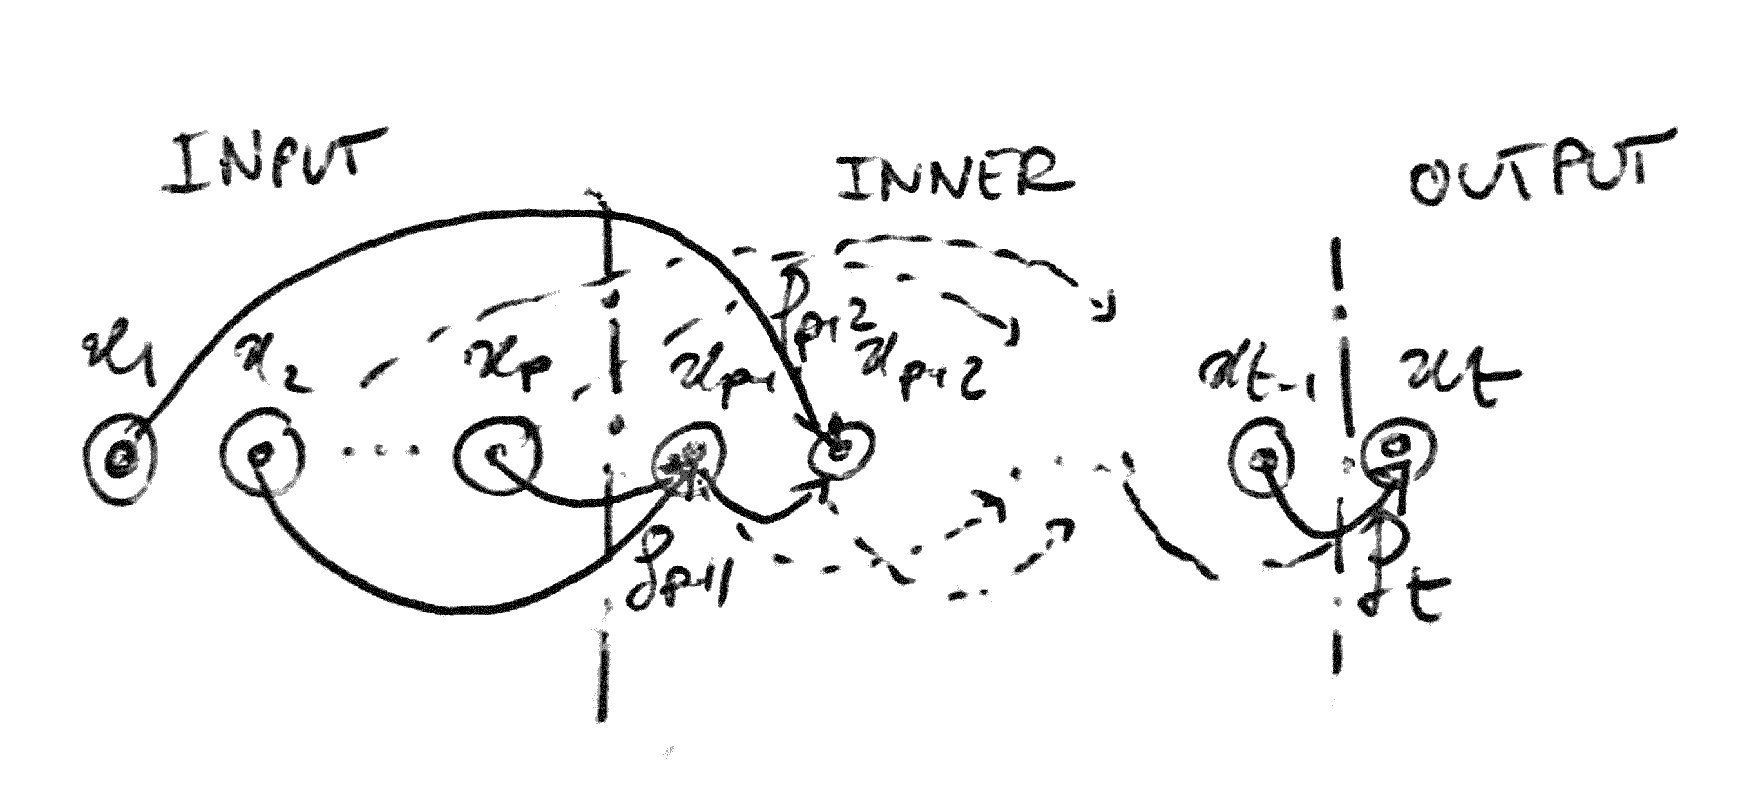
\includegraphics[width=.5\linewidth]{auto-diff/comp-graph}
\caption{\label{fig-compgraph}
A computational graph.
}
\end{figure}

A numerical algorithm can be represented as a succession of functions of the form
\eq{
	\foralls k=s+1,\ldots,t, \quad x_k = f_k( x_1,\ldots,x_{k-1} )
}
where $f_k$ is a function which only depends on the previous variables, see Fig.~\ref{fig-compgraph}. One can represent this algorithm using a directed acyclic graph (DAG), linking the variables involved in $f_k$ to $x_k$. The node of this graph are thus conveniently ordered by their indexing, and the directed edges only link a variable to another one with a strictly larger index.
%
The evaluation of $f(x)$ thus corresponds to a forward traversal of this graph. 



%%%%%%%%%%%%%%%%%%%%%%%%%%%%%%%%%%%%%%%%%%%%%%%%%%%%%%%%%%%%%%%%%%%%%%%%
\subsection{Forward Mode of Automatic Differentiation}

The forward mode correspond to the usual way of computing differentials. It compute the derivative $\pd{x_k}{x_1}$ of all variables $x_k$ with respect to $x_1$. One then needs to repeat this method $p$ times to compute all the derivative with respect to $x_1,x_2,\ldots,x_p$ (we only write thing for the first variable, the method being of course the same with respect to the other ones).



\newcommand{\bk}[1]{\left[#1\right]}
\newcommand{\pdb}[2]{\bk{\pd{#1}{#2}}}

\wrapfSimple{auto-diff/forward-mode.pdf}
The method initialize the derivative of the input nodes 
\eq{
	\pd{x_1}{x_1} = \Id_{n_1 \times n_1}, \quad 
	\pd{x_2}{x_1} = 0_{n_2 \times n_1}, \ldots, \quad
	\pd{x_s}{x_1} = 0_{n_s \times n_1}, 
}
(and thus 1 and 0's for scalar variables), and then iteratively make use of the following recursion formula
\eq{
	\foralls k=s+1,\ldots,t, \quad
	\pd{x_k}{x_1} 
	= \sum_{\ell \in \text{father}(k)} \bk{\pd{x_k}{x_\ell}} \times \pd{x_\ell}{x_1}
	= \sum_{\ell \in \text{father}(k)} \pd{f_k}{x_\ell}(x_1,\ldots,x_{k-1}) \times \pd{x_\ell}{x_1}.
}

The notation ``$\text{father}(k)$'' denotes the nodes $\ell<k$ of the graph that are connected to $k$.
%
Here the quantities being computed (i.e. stored in computer variables) are the derivatives $\pd{x_\ell}{x_1}$, and $\times$ denotes in full generality matrix-matrix multiplications.
%
We have put in $[\ldots]$ an informal notation, since here $\pd{x_k}{x_\ell}$ should be interpreted not as a numerical variable but needs to be interpreted as derivative of the function $f_k$, which can be evaluated on the fly (we assume that the derivative of the function involved are accessible in closed form).  

Assuming all the involved functions $\pd{f_k}{x_k}$ have the same complexity (which is likely to be the case if all the $n_k$ are for instance scalar or have the same dimension), and that the number of father node is bounded, one sees that the complexity of this scheme is $p$ times the complexity of the evaluation of $f$ (since this needs to be repeated $p$ times for $\pd{}{x_1},\ldots,\pd{}{x_p}$). For a large $p$, this is prohibitive. 

\begin{figure}
\centering
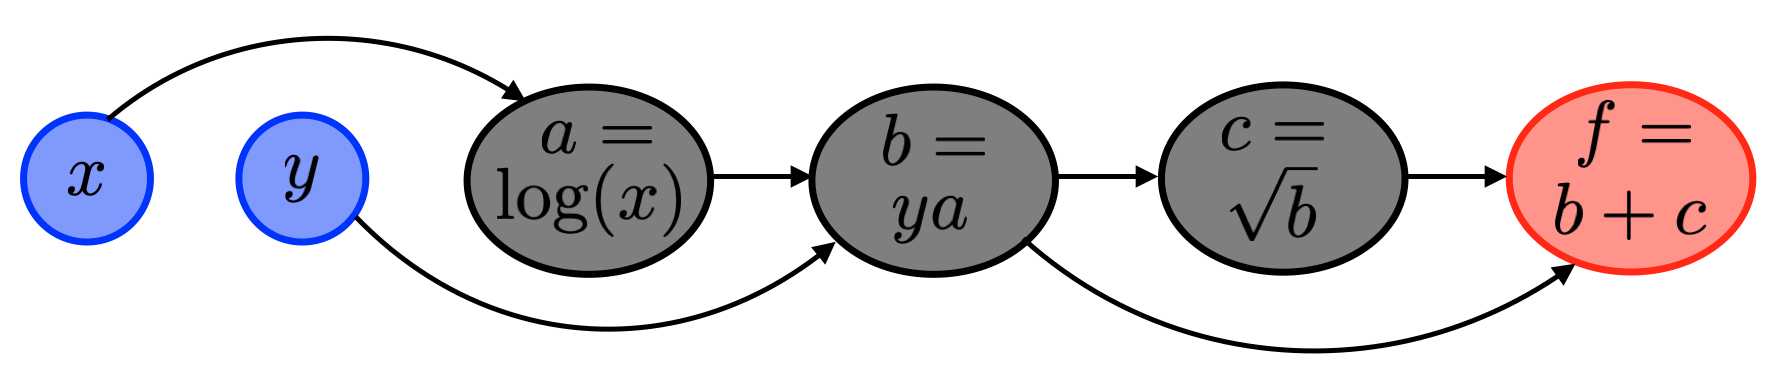
\includegraphics[width=.6\linewidth]{auto-diff/example-simple}
\caption{\label{fig-dag-example-simple}
Example of a simple computational graph.
}
\end{figure}




%%%
\paragraph{Simple example.}

We consider the fonction 
\eql{\label{eq-simple-func-autodiff}
 	f(x) = \log(x)+\sqrt{\log(x)}
} 
whose computational graph is displayed on Figure~\ref{fig-dag-example-simple}. The iterations of the forward mode read
\begin{align*}
		\pd{x}{x} &= 1 \\
		\pd{y}{x} &= \bk{\pd{y}{x}} \pd{x}{x} = \frac{1}{x} \pd{x}{x} &
			\{x \mapsto y = \log(x)\}\\
		\pd{z}{x} &= \bk{\pd{z}{y}} \pd{y}{x} = \frac{1}{2\sqrt{y}} \pd{y}{x} &
			\{y \mapsto z=\sqrt{y}\}\\
		\pd{f}{x} &= \bk{\pd{f}{z}} \pd{z}{x} + \bk{\pd{f}{y}} \pd{y}{x} = 1 \pd{z}{x} + 1 \pd{y}{x}&
			\{(x,z) \mapsto f=x+z\}
\end{align*}



\begin{figure}
\centering
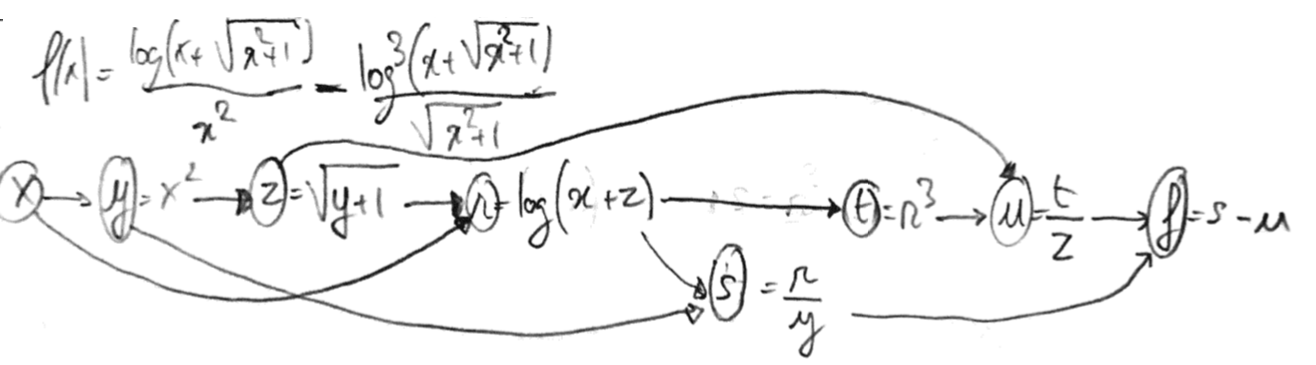
\includegraphics[width=.6\linewidth]{auto-diff/example-complex}
\caption{\label{fig-dag-example-complex}
Example of a more complex computational graph.
}
\end{figure}

%%%
\paragraph{More complex example.}

We now consider the fonction 
\eql{\label{eq-cpx-func-autodiff}
	f(x) = \frac{\log(x+\sqrt{x^2+1})}{x^2} - \frac{\log^3(x+\sqrt{x^2+1})}{\sqrt{x^2+1}}
}
whose computational graph is displayed on Figure~\ref{fig-dag-example-complex}. The iterations of the forward mode read
\begin{align*}
		\pd{x}{x} &= 1 \\
		\pd{y}{x} &= \pdb{y}{x} \pd{x}{x}  = 2 x \pd{x}{x}  &
			\{x \mapsto y = x^2\} \\
		\pd{z}{x} &= \pdb{z}{y} \pd{y}{x} = \frac{1}{2\sqrt{y+1}} \pd{y}{x} &
			\{y \mapsto z=\sqrt{y+1}\}\\
		\pd{r}{x} &= \pdb{r}{z} \pd{x}{x} + \pdb{r}{z} \pd{z}{x} = \frac{1}{x+r} \pd{x}{x} + \frac{1}{x+r} \pd{z}{x}&
			\{(x,z) \mapsto r=\log(x+z)\} \\
		\pd{s}{x} &= \pdb{s}{r} \pd{r}{x} + \pdb{s}{y}\pd{y}{x} = \frac{1}{y} \pd{r}{x} - \frac{r}{y^2}\pd{y}{x} &
			\{ (r,y) \mapsto s=\frac{r}{y}  \} \\
		\pd{t}{x} &= \pdb{t}{r} \pd{r}{x} = 3r^2 \pd{r}{x} &
			\{ r \mapsto t = r^3 \} \\
		\pd{u}{x} &= \pdb{u}{t} \pd{t}{x} + \pdb{u}{z}\pd{z}{x} = \frac{1}{z} \pd{t}{x} - \frac{t}{z^2} \pd{z}{x} &
			\{ (t,z) \mapsto u =  \frac{t}{z}  \} \\
		\pd{f}{x} &= \pdb{f}{s}\pd{s}{x} + \pdb{f}{u}\pd{u}{x} = 1 \pd{s}{x} - 1 \pd{u}{x} &
			\{ (s,u) \mapsto f = s-u \}
\end{align*}



%%%%%%%%%%%%%%%%%%%%%%%%%%%%%%%%%%%%%%%%%%%%%%%%%%%%%%%%%%%%%%%%%%%%%%%%
\subsection{Reverse Mode of Automatic Differentiation}

Instead of evaluating the differentials $\pd{x_k}{x_1}$ which is problematic for a large $p$, the reverse mode evaluates the differentials  $\pd{x_t}{x_k}$, i.e. it computes the derivative of the output node with respect to the all the inner nodes. 

\wrapfSimple{auto-diff/backward-mode.pdf}
The method initialize the derivative of the final node
\eq{
	\pd{x_t}{x_t} = \Id_{n_t \times n_t}, 
}
and then iteratively makes use,  from the last node to the first, of the following recursion formula
\eq{
	\foralls k=t-1,t-2,\ldots,1, \quad
	\pd{x_t}{x_k} 
	= \sum_{m \in \text{son}(k)}  \pd{x_t}{x_m} \times \bk{\pd{x_m}{x_k}}
	= \sum_{m \in \text{son}(k)} \pd{x_t}{x_m} \times \pd{f_m(x_1,\ldots,x_m)}{x_k}.
}
%
The notation ``$\text{father}(k)$'' denotes the nodes $\ell<k$ of the graph that are connected to $k$.

%%%
\paragraph{Back-propagation.}

In the special case where $x_t \in \RR$, then $\pd{x_t}{x_k} = [\nabla_{x_k} f(x)]^\top \in \RR^{1 \times n_k}$ and one can write the recursion on the gradient vector as follow 
\eq{
	\foralls k=t-1,t-2,\ldots,1, \quad
	\nabla_{x_k} f(x) 
	= \sum_{m \in \text{son}(k)} \pa{\pd{f_m(x_1,\ldots,x_m)}{x_k}}^\top \pa{
	 	\nabla_{x_m} f(x)
	}.
}
where $\pa{\pd{f_m(x_1,\ldots,x_m)}{x_k}}^\top \in \RR^{n_k \times n_m}$ is the adjoint of the Jacobian of $f_m$. This form of recursion using adjoint is often referred to as ``back-propagation'', and is the most frequent setting in applications to ML.

In general, when $n_t=1$, the backward is the optimal way to compute the gradient of a function. Its drawback is that it necessitate the pre-computation of all the intermediate variables $(x_k)_{k=p}^t$, which can be prohibitive in term of memory usage when $t$ is large. There exists check-pointing method to alleviate this issue, but it is out of the scope of this course.

%%%
\paragraph{Simple example.}

We consider once again the fonction $f(x)$ of~\eqref{eq-simple-func-autodiff}, the iterations of the reverse mode read
\begin{align*}
		\pd{f}{f} &= 1 &\\
		\pd{f}{z} &= \pd{f}{f} \pdb{f}{z} = \pd{f}{f} 1 &
			\{z \mapsto f = x+z\}\\
		\pd{f}{y} &= \pd{f}{z} \pdb{z}{y} + \pd{f}{f} \pdb{f}{y} = \pd{f}{z} \frac{1}{2\sqrt{y}} + \pd{f}{f} 1 & 
			\{ y \mapsto z=\sqrt{y}, y \mapsto f=y+z\} \\
		\pd{f}{x} &= \pd{f}{y} \pdb{y}{x} = \pd{f}{y} \frac{1}{x} & 
			\{ x \mapsto y=\log(x)\}
\end{align*}

%%%
\paragraph{More complex example.}

We consider once again the fonction $f(x)$ of~\eqref{eq-cpx-func-autodiff}, the iterations of the reverse mode read
\begin{align*}
		\pd{f}{f} &= 1 &\\
		\pd{f}{u} &= \pd{f}{f} \pdb{f}{u} 
			= \pd{f}{f} (-1) &
			\{u \mapsto f = s-u\}\\
		\pd{f}{t} &= \pd{f}{u} \pdb{u}{t} 
			= \pd{f}{u} \frac{1}{z}  & 
			\{ t \mapsto u= \sqrt{y}, y \frac{t}{z} \} \\
		\pd{f}{s} &= \pd{f}{f} \pdb{f}{s} = \pd{f}{f} 1 & 
			\{ s \mapsto f = s-u \} \\
		\pd{f}{r} &= \pd{f}{t} \pdb{t}{r} + \pd{f}{s} \pdb{s}{r} 
			= \pd{f}{t} 3r^2 + \pd{f}{s} \frac{1}{y} & 
			\{ r \mapsto s = \frac{r}{y}, r \mapsto  t=r^3\}  \\
		\pd{f}{z} &= \pd{f}{u} \pdb{u}{z} + \pd{f}{r} \pdb{r}{z} 
			= \pd{f}{u} \frac{-t}{z^2} + \pd{f}{r} \pdb{1}{x+z} &
			\{ z \mapsto u=\frac{t}{z}, z \mapsto r=\log(x+z)\} \\
		\pd{f}{y} &= \pd{f}{z}\pdb{z}{y} + \pd{f}{s}\pdb{s}{y}
			= \pd{f}{z} \frac{1}{2\sqrt{y+1}} + \pd{f}{s}\frac{-r}{y^2} &
			\{ y \mapsto z=\sqrt{y+1}, y \mapsto s = \frac{r}{y}\} \\
		\pd{f}{x} &= \pd{f}{y}\pdb{y}{x} + \pd{f}{r}\pdb{r}{x}
			= \pd{f}{y} 2x + \pd{f}{r} \frac{1}{x+z}  &
			\{x \mapsto y=x^2, x \mapsto r=\log(x+z)\}		
\end{align*}



%%%%%%%%%%%%%%%%%%%%%%%%%%%%%%%%%%%%%%%%%%%%%%%%%%%%%%%%%%%%%%%%%%%%%%%%
\subsection{Feed-forward Architectures}

The simplest computational graphs are purely feedforward, and corresponds to the computation of 
\eql{\label{eq-simple-lin-dag}
	f = f_{t-1} \circ f_{t-2} \circ \ldots \circ f_2 \circ f_1
}
for functions $f_k : \RR^{n_k} \rightarrow \RR^{n_{k+1}}$.

The forward function evaluation algorithm initializes $x_0=x$ and then computes
\eq{
	\foralls k=1, \ldots, t-1, \quad x_{k+1} = f_k(x_k)
}
where at the output, one retrieves $f(x) = x_t$.

Denoting $A_k \eqdef \partial f_k(x_k) \in \RR^{n_{k+1} \times n_k}$ the Jacobian, one has
\eq{
	\partial f(x) = A_{t-1} \times A_{t-2} \times \ldots A_2 \times A_1.
}
The forward (resp. backward) mode corresponds to the computation of the product of the Jacobian from right to left (resp. left to right) 
\begin{align*}
	\partial f(x) &= A_{t-1} \times \pa{  A_{t-2} \times \pa{ \ldots \times \pa{ A_3 \times \pa{ A_2 \times A_1 } } } }, \\
	\partial f(x) &= \pa{ \pa{ \pa{ \pa{ A_{t-1} \times A_{t-2} }  \times A_{t-3} } \times \ldots } \times A_2 } \times A_1.
\end{align*}


\begin{figure}
\centering
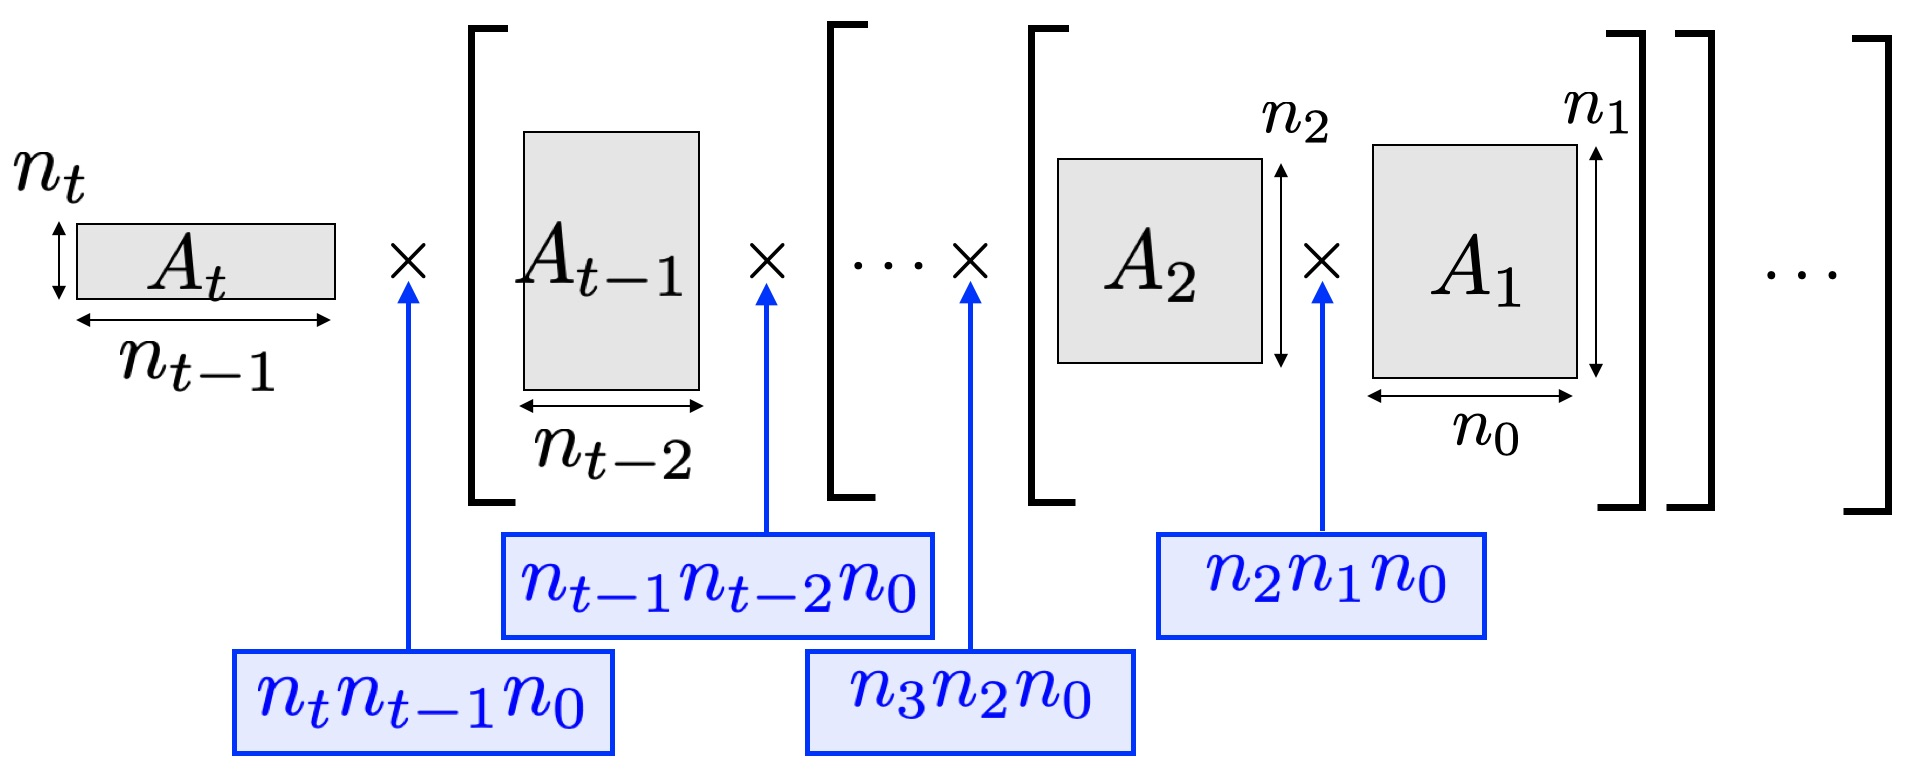
\includegraphics[width=.35\linewidth]{auto-diff/matrix-forward} 
\quad\quad
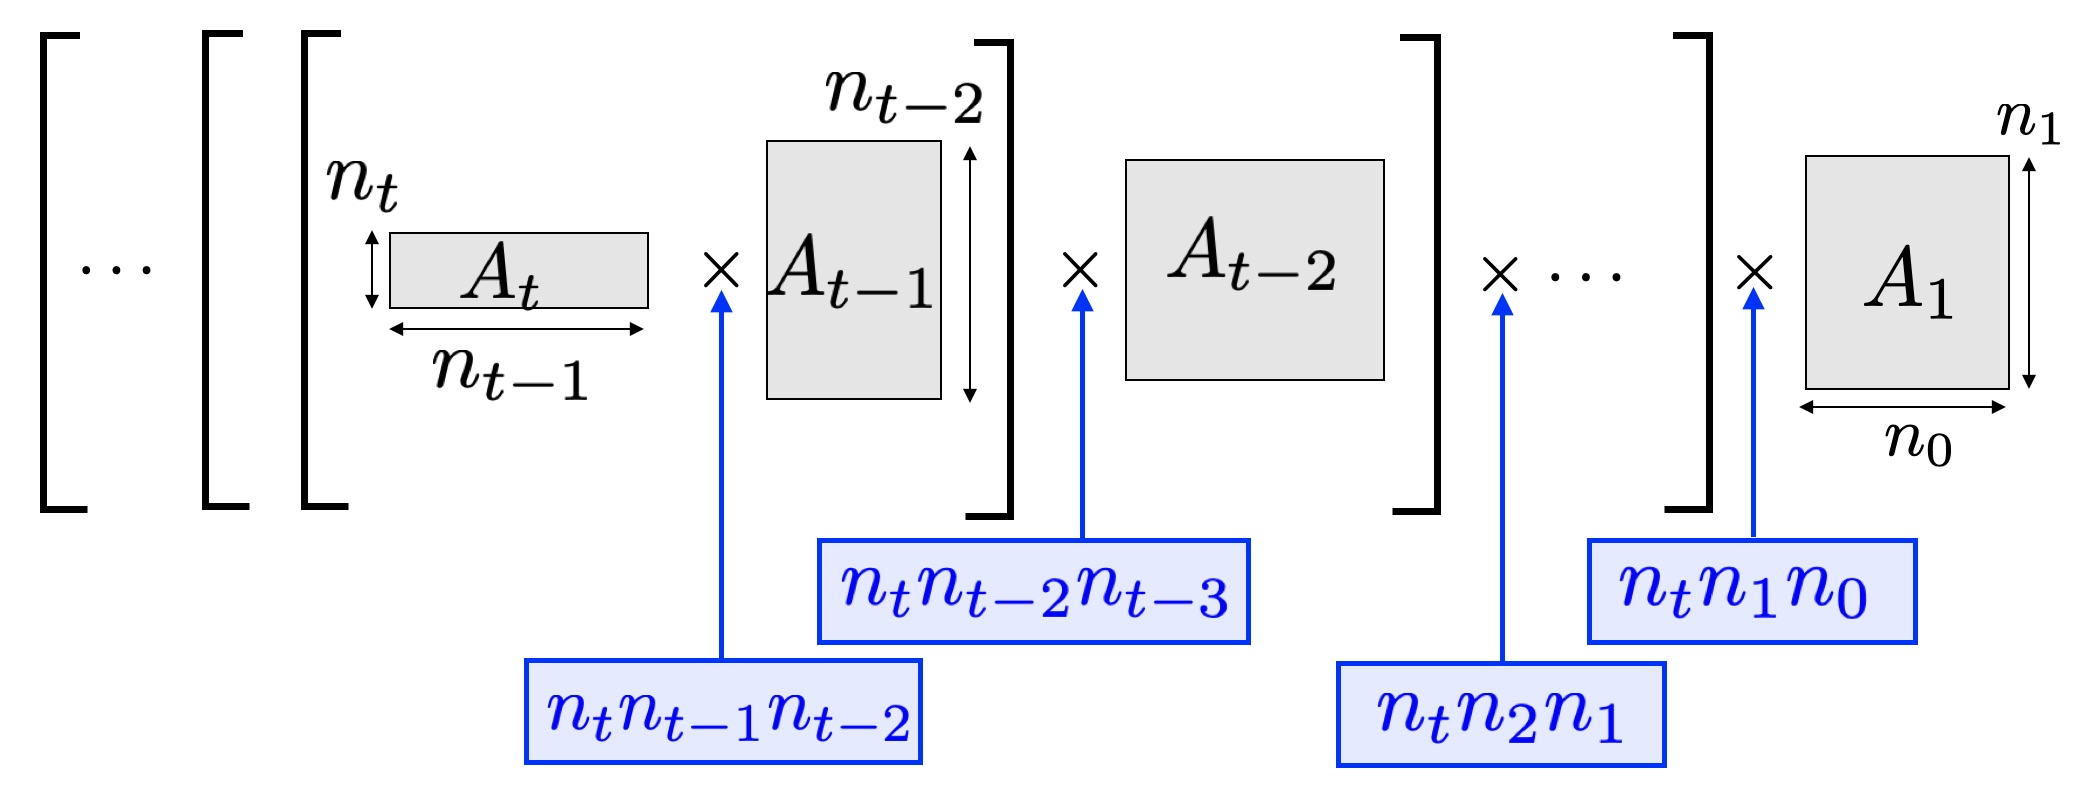
\includegraphics[width=.35\linewidth]{auto-diff/matrix-backward} 
\caption{\label{fig-matrix-mult}
Complexity of forward (left) and backward (right) modes for feedforward graphs.
}
\end{figure}

We note that the computation of the product $A \times B$ of $A \in \RR^{n \times p}$ with $B \in \RR^{p \times q}$ necessitates $npq$ operations.
%
As shown on Figure~\ref{fig-matrix-mult}, the complexity of the forward and backward modes are
\eq{
	n_1 \sum_{k=2}^{t-1} n_k n_{k+1}
	\qandq
	n_t \sum_{k=1}^{t-2} n_k n_{k+1}
}
So if $n_t \ll n_1$ (which is the typical case in ML scenario where $n_t=1$) then the backward mode is cheaper. 




%%%%%%%%%%%%%%%%%%%%%%%%%%%%%%%%%%%%%%%%%%%%%%%%%%%%%%%%%%%%%%%%%%%%%%%%
\subsection{Multilayer Perceptron}
\label{sec-autodiff-mlp}


We consider a feedforward deep network (fully connected for simplicity), initialized as $a_0=a$ and defined through 
\eql{\label{eq-mlp-def}
	\foralls k=1,\ldots,t, \quad \choice{
		b_k \eqdef W_k a_{k-1} \\
		a_k \eqdef \rho(b_k) 
		}
} 
where $\rho$ is a point wise non-linearity (so $\rho(u)$ actually denoted $(\rho(u_i))_i$), $W_k \in \RR^{n_k \times n_{k-1}}$ are the weight to be trained, and the final output is set as, for $W=(W_1,\ldots,W_t)$, 
\eq{
	f(W) \eqdef \ell(b_t,y)
}
where $\ell : \RR \times \RR \rightarrow 0$ is some loss function. Figure~\ref{fig-mlp} displays the computational graph.

The backward automatic differentiation method (aka back-propagation) proceeds by first computing the $(a_k)_{k=1}^t$ by forward evaluation, and then intializing the gradient vector
\eq{
	\nabla_{b_t} f = \ell'(b_t,y)
}
where $\ell'$ is the derivative with respect to the first variable, and then applying the adjoint on the chain rule of $a_{k-1} \mapsto b_k  = W_k a_{k-1}\mapsto a_k = \rho(b_k)$
\begin{align*}
	\nabla_{b_{k}} f &= \diag(\rho'(b_k)) \nabla_{a_k} f \\
	\nabla_{a_{k-1}} f &= W_k^\top b_{k}
\end{align*}
The gradient of with respect to the weight matrices are obtained by also applying the adjoint on the chain rule, but this time to of $W_k \mapsto b_k  = W_k a_{k-1}$
 \eq{
 	\nabla_{W_{k}} f = (\nabla_{b_k} f) a_{k-1}^\top.
}


\begin{figure}
\centering
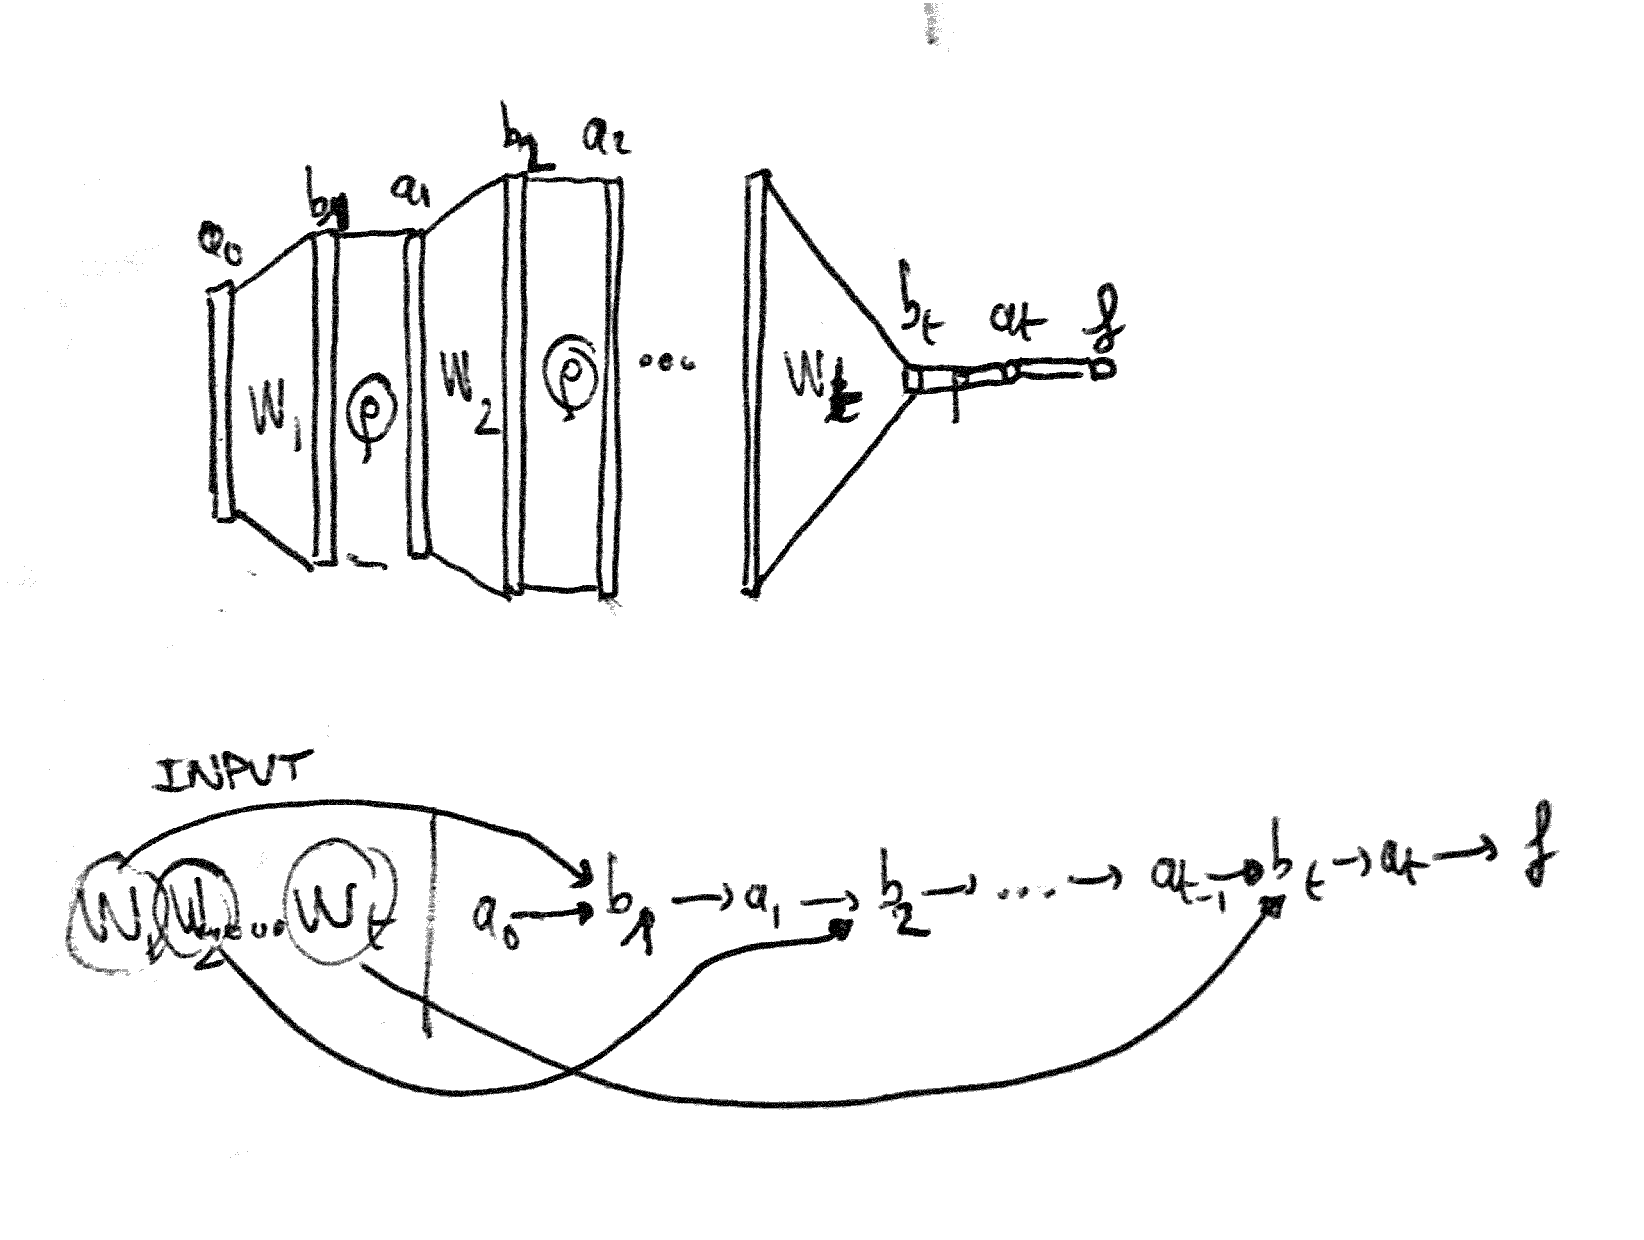
\includegraphics[width=.6\linewidth]{auto-diff/mlp.pdf} 
\caption{\label{fig-mlp}
Computational graph for a MLP.
}
\end{figure}


